%
% Komponenten
% Abschlussarbeit (Bachelor)
%
% Thema: Erstellung einer Browser Extension zur Usability Evaluierung von beliebigen Web-Applikationen über Heatmaps.
% Betreuer 1: Prof. Dr. Targo Pavlista
% Betreuer 2: Siamak Haschemi
%
% @author Christian Bromann <contact@christian-bromann.com>
%

\section{Komponenten}

Der Aufbau von \textit{thEvaluator} besteht aus drei Komponenten. Darunter gehören eine Web-Applikation, die es ermöglicht, Testcases zu erstellen und zu verwalten, eine API und Socket-Schnittstelle, die sich um die Persistierung und Ausgabe jeglicher Daten kümmert, sowie einer Browser Extension für den Chrome Browser, die den User durch den Test führt. Abbildung \ref{structure} zeigt, wie diese einzelnen Komponenten miteinander arbeiten. Datenpakete werden dabei entweder via Socket Verbindung oder Ajax Request ausgetauscht.

\begin{center}
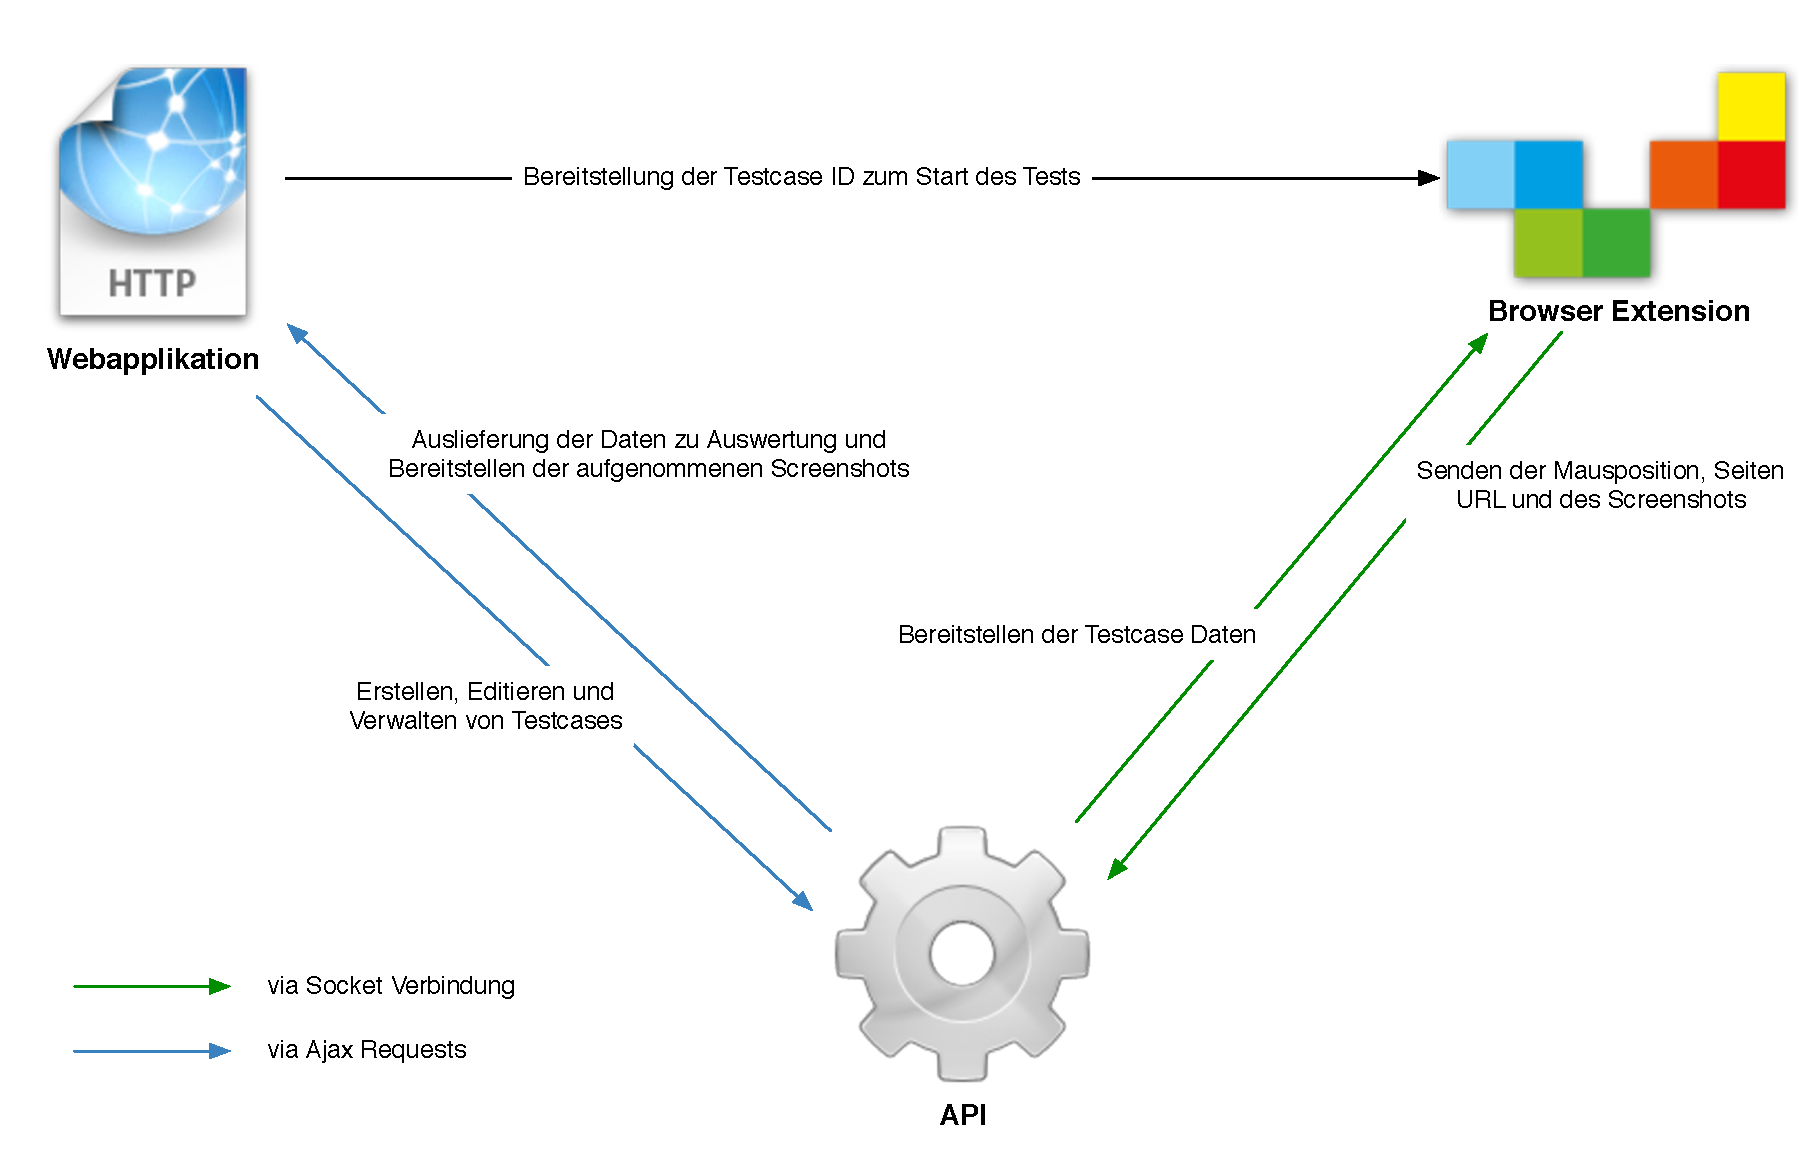
\includegraphics[scale=0.5]{./images/structure}
\end{center}
\begin{figure}[htb]
   \centering
   \caption{Zusammenwirken der einzelnen Komponenten des \textit{thEvaluator} Frameworks}
    \label{structure}
\end{figure}
\newpage